%%%%%%%%%%%%%%%%%%%%%%%%%%%%%%%%%%%%%%%%%%%%%%%%%%%%%%%%%%%%%%%%%%%%%%%%%%%%%%%%
%                    Capitulo 7: Diseño software del sistema                   %
%%%%%%%%%%%%%%%%%%%%%%%%%%%%%%%%%%%%%%%%%%%%%%%%%%%%%%%%%%%%%%%%%%%%%%%%%%%%%%%%

\chapter{Diseño \textit{software} del sistema}

\section{Implementación}

El sistema completo ha sido implementado utilizando \texttt{Python} y \texttt{Java}.
El primer lenguaje se ha utilizado para crear el \textit{script} que permite
automatizar la generación de archivos de configuración plantilla, mientras que el segundo
se ha utilizado para implementar el resto de la arquitectura, ya que el entorno
\texttt{GVG-AI} fue originalmente escrito en \texttt{Java}. Todo el código fuente
se encuentra disponible en un repositorio público de \texttt{GitHub}, con lo cual
cualquiera puede acceder a él.

Si se desean consultar más detalles sobre la implementación, se recomienda consultar
el documento adjunto, el cual contiene más información.

\section{Arquitectura \textit{software} del sistema}

El sistema se ha implementado mediante una serie de clases, las cuales posteriormente
se han agrupado en un paquete, creando por tanto un módulo \textit{software}. En el diagrama
de clases de la figura \ref{fig:class_diagram} se puede observar qué clases componen
el paquete, cuáles son las relaciones entre ellas, qué información guardan y
qué funcionalidades exponen.

\begin{figure}[H]
    \centering
    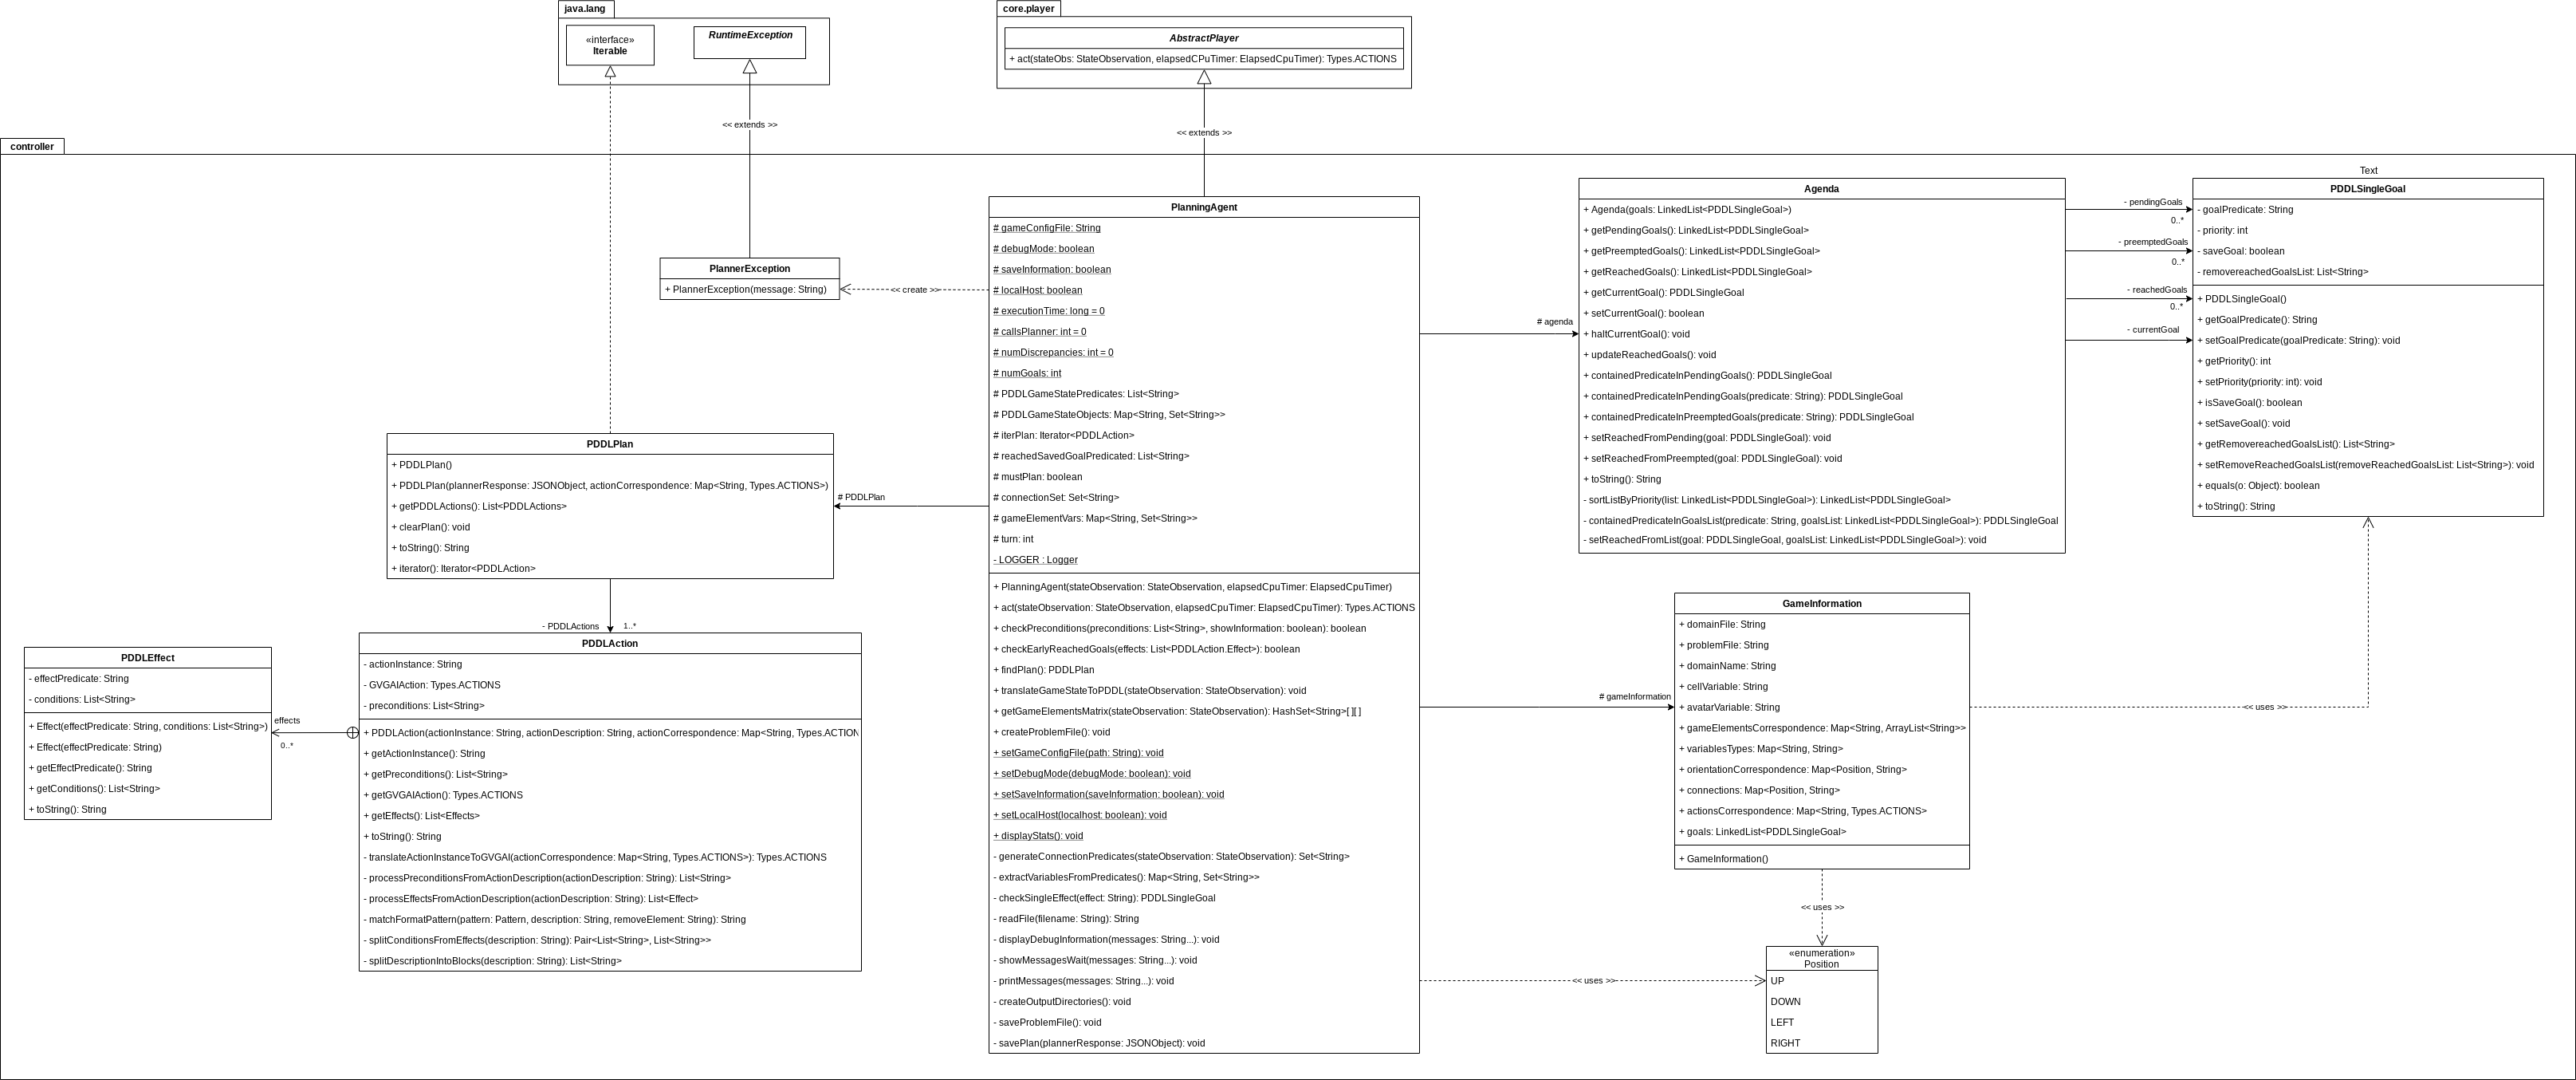
\includegraphics[angle=90, origin=c, scale=0.18]{img/CH07/class_diagram.png}
    \caption{Diagrama de clases.}
    \label{fig:class_diagram}
\end{figure}

\begin{figure}[H]
    \centering
    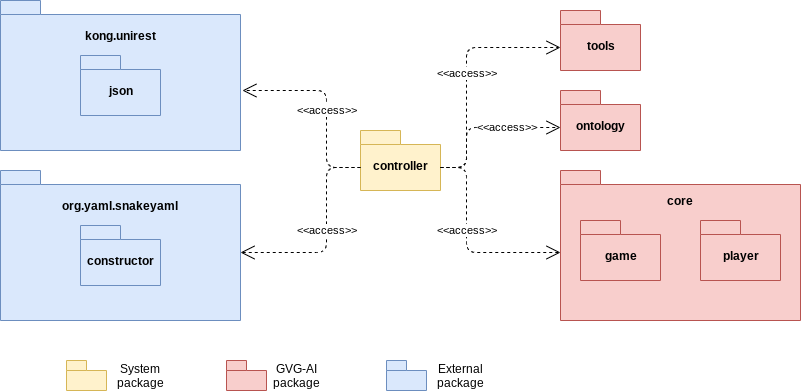
\includegraphics[scale=0.48]{img/CH07/package_diagram.png}
    \caption{Diagrama de paquetes.}
    \label{fig:package_diagram}
\end{figure}

En la figura \ref{fig:package_diagram} se puede apreciar cómo se relaciona el paquete
que encapsula el sistema, \texttt{controller}, con otros paquetes. Puede verse que el paquete del sistema
accede a las funcionalidades que se pueden encontrar en algunos de los paquetes que ofrece el entorno de
\texttt{GVG-AI}. También se puede observar que se accede a funcionalidad de módulos externos, como por
ejemplo a \texttt{kong.unirest} y a su subpaquete \texttt{json} y al paquete \texttt{org.yaml.snakeyaml}
y a su subpaquete \texttt{constructor}.

El paquete \texttt{kong.unirest} junto con su subpaquete \texttt{json} se han utilizado
para hacer las peticiones al planificador, el cual ha sido comentado varias veces que es un componente
que se encuentra desplegado en la nube, y que por tanto, ofrece una \texttt{API REST} a la cual se
pueden hacer peticiones utilizando los métodos de \texttt{HTTP}.

El paquete \texttt{org.yaml.snakeyaml} junto con su subpaquete \texttt{constructor} se han
utilizado para cargar el archivo de configuración en formato \texttt{YAML} a la correspondiente
estructura de datos que se ha definido.

\section{Descripción de las clases}

Una vez que se ha visto cómo se ha estructurado el módulo \textit{software}, vamos
a pasar a comentar de forma general las clases que lo conforman.

\subsection{La clase \texttt{PlanningAgent}}

Esta es la clase que representa el agente implementado, el cual combina una componente deliberativa
(la planificación) con una componente reactiva (el monitor). Hereda de la clase abstracta
\texttt{AbstractPlayer}, la cual es proporcionada por el entorno de \texttt{GVG-AI}. Como
tal no se instancia si no que se le indica al entorno la ruta de la clase que se quiere ejecutar.
Si se quiere configurar de alguna forma o acceder a las estadísticas una vez se ha completado
el juego, se deben utilizar los métodos estáticos proporcionados (ver figura \ref{fig:class_diagram}).

Aparte de disponer de atributos de configuración y de estadísticas, la clase dispone de un \textit{logger}
(atributo \texttt{LOGGER}) que permite guardar información de la ejecución en un \textit{log} si
se especifica la opción a la hora de ejecutar el sistema.

La mayoría de atributos están bastante claros, aunque se quieren destacar los siguientes, los cuales
son de especial interés:

\begin{itemize}[label=\textbullet]
    \item \texttt{PDDLGameStatePredicates}: Lista que contiene todos los predicados \texttt{PDDL} del estado
    actual del juego. Estos predicados están asociados a las observaciones del juego y a las relaciones
    de conectividad entre las casillas.
    
    \item \texttt{PDDLGameStateObjects}: Diccionario que relaciona las variables definidas en el archivo
    de configuración con los objetos del juego que se han construido utilizando dicha variable (instancias
    concretas de la variable).
    
    \item \texttt{iterPlan}: Iterador que permite recorrer de forma sencilla el plan generado.
    
    \item \texttt{reachedSavedGoalPredicates}: Lista de predicados objetivo alcanzados que deben
    ser añadidos a los predicados del estado actual.
    
    \item \texttt{mustPlan}: Variable booleana que indica si se debe planificar o no.
    
    \item \texttt{connectionSet}: Conjunto que contiene los predicados asociados a las relaciones
    de conectividad de las celdas. Estos predicados se tienen guardados aparte ya que solo se
    generan una vez al principio de la partida y posteriormente se añaden a \texttt{PDDLGameStatePredicates}.
    
    \item \texttt{gameElementVars}: Diccionario que relaciona los elementos del juego y las
    variables asociadas a estos elementos.
\end{itemize}

De entre los métodos disponibles, se quieren comentar algunos de ellos debido a que
son de especial importancia:

\begin{itemize}[label=\textbullet]
    \item \texttt{act}: Este es el método más importante de la clase y de todo el sistema. Se ejecuta
    en cada turno y devuelve la siguiente acción que tiene que ejecutar el agente. Podría considerarse que
    es el \textbf{ejecutor del plan} del sistema, ya que es el que manda las acciones a ejecutar
    al motor del juego. Se encarga también de comunicarse con todos los demás módulos funcionales que se
    han descrito en los capítulos \ref{chap:arch} y \ref{chap:desc} para determinar la siguiente acción a
    ejecutar. Su funcionamiento puede verse en el diagrama de secuencia de la figura \ref{fig:sequence_diagram},
    donde se muestra cómo se comunica con los otros elementos.
    
    \item \texttt{checkPreconditions}: Este método es una parte del \textbf{monitor}, encargándose de
    determinar si se ha producido una discrepancia debido a que no se cumplen las precondiciones
    de una acción.
    
    \item \texttt{checkEarlyReachedGoals}: La otra parte del \textbf{monitor}, encargándose de
    comprobar si algún objetivo se ha alcanzado antes de tiempo.
    
    \item \texttt{findPlan}: En este método se lleva a cabo la llamada al planificador, lo que se
    correspondería la tarea realizada por el \textbf{planificador}. Dentro de él también se realiza
    la traducción del plan, aunque no es una tarea que realiza este método directamente.
    
    \item \texttt{translateGameStateToPDDL}: Este método traduce el estado de observación actual del juego
    a predicados \texttt{PDDL}, aunque solo lo hace para las observaciones. También añadiría los predicados
    que se encuentran en el atributo \texttt{reachedSavedGoalPredicated}. Por tanto, realiza una parte
    del trabajo que realiza el \textbf{traductor del estado de observación}.
    
    \item \texttt{generateConnectionPredicates}: Este método genera los predicados que representan
    las relaciones de conectividad entre las celdas. Por tanto, realizaría parte del funcionamiento
    del \textbf{traductor del estado de observación}.
    
    \item \texttt{getGameElementsMatrix}: Este método transforma el estado de observación que es
    proporcionado por el motor del juego a una matriz que contiene los nombres de los elementos del
    juego en cada posición. Puede haber más de un elemento en una misma posición. Estos nombres se
    corresponden con los que hay en el archivo de configuración. Este método es indispensable para
    que se pueda hacer correctamente la traducción de los estados de observación. Realiza, por tanto,
    una parte del trabajo del \textbf{traductor del estado de observación}.
    
    \item \texttt{createProblemFile}: Este método genera el archivo de problemas. Por tanto, su
    funcionamiento se corresponde con el descrito para el \textbf{generador de problemas}.
\end{itemize}

\begin{figure}[H]
    \centering
    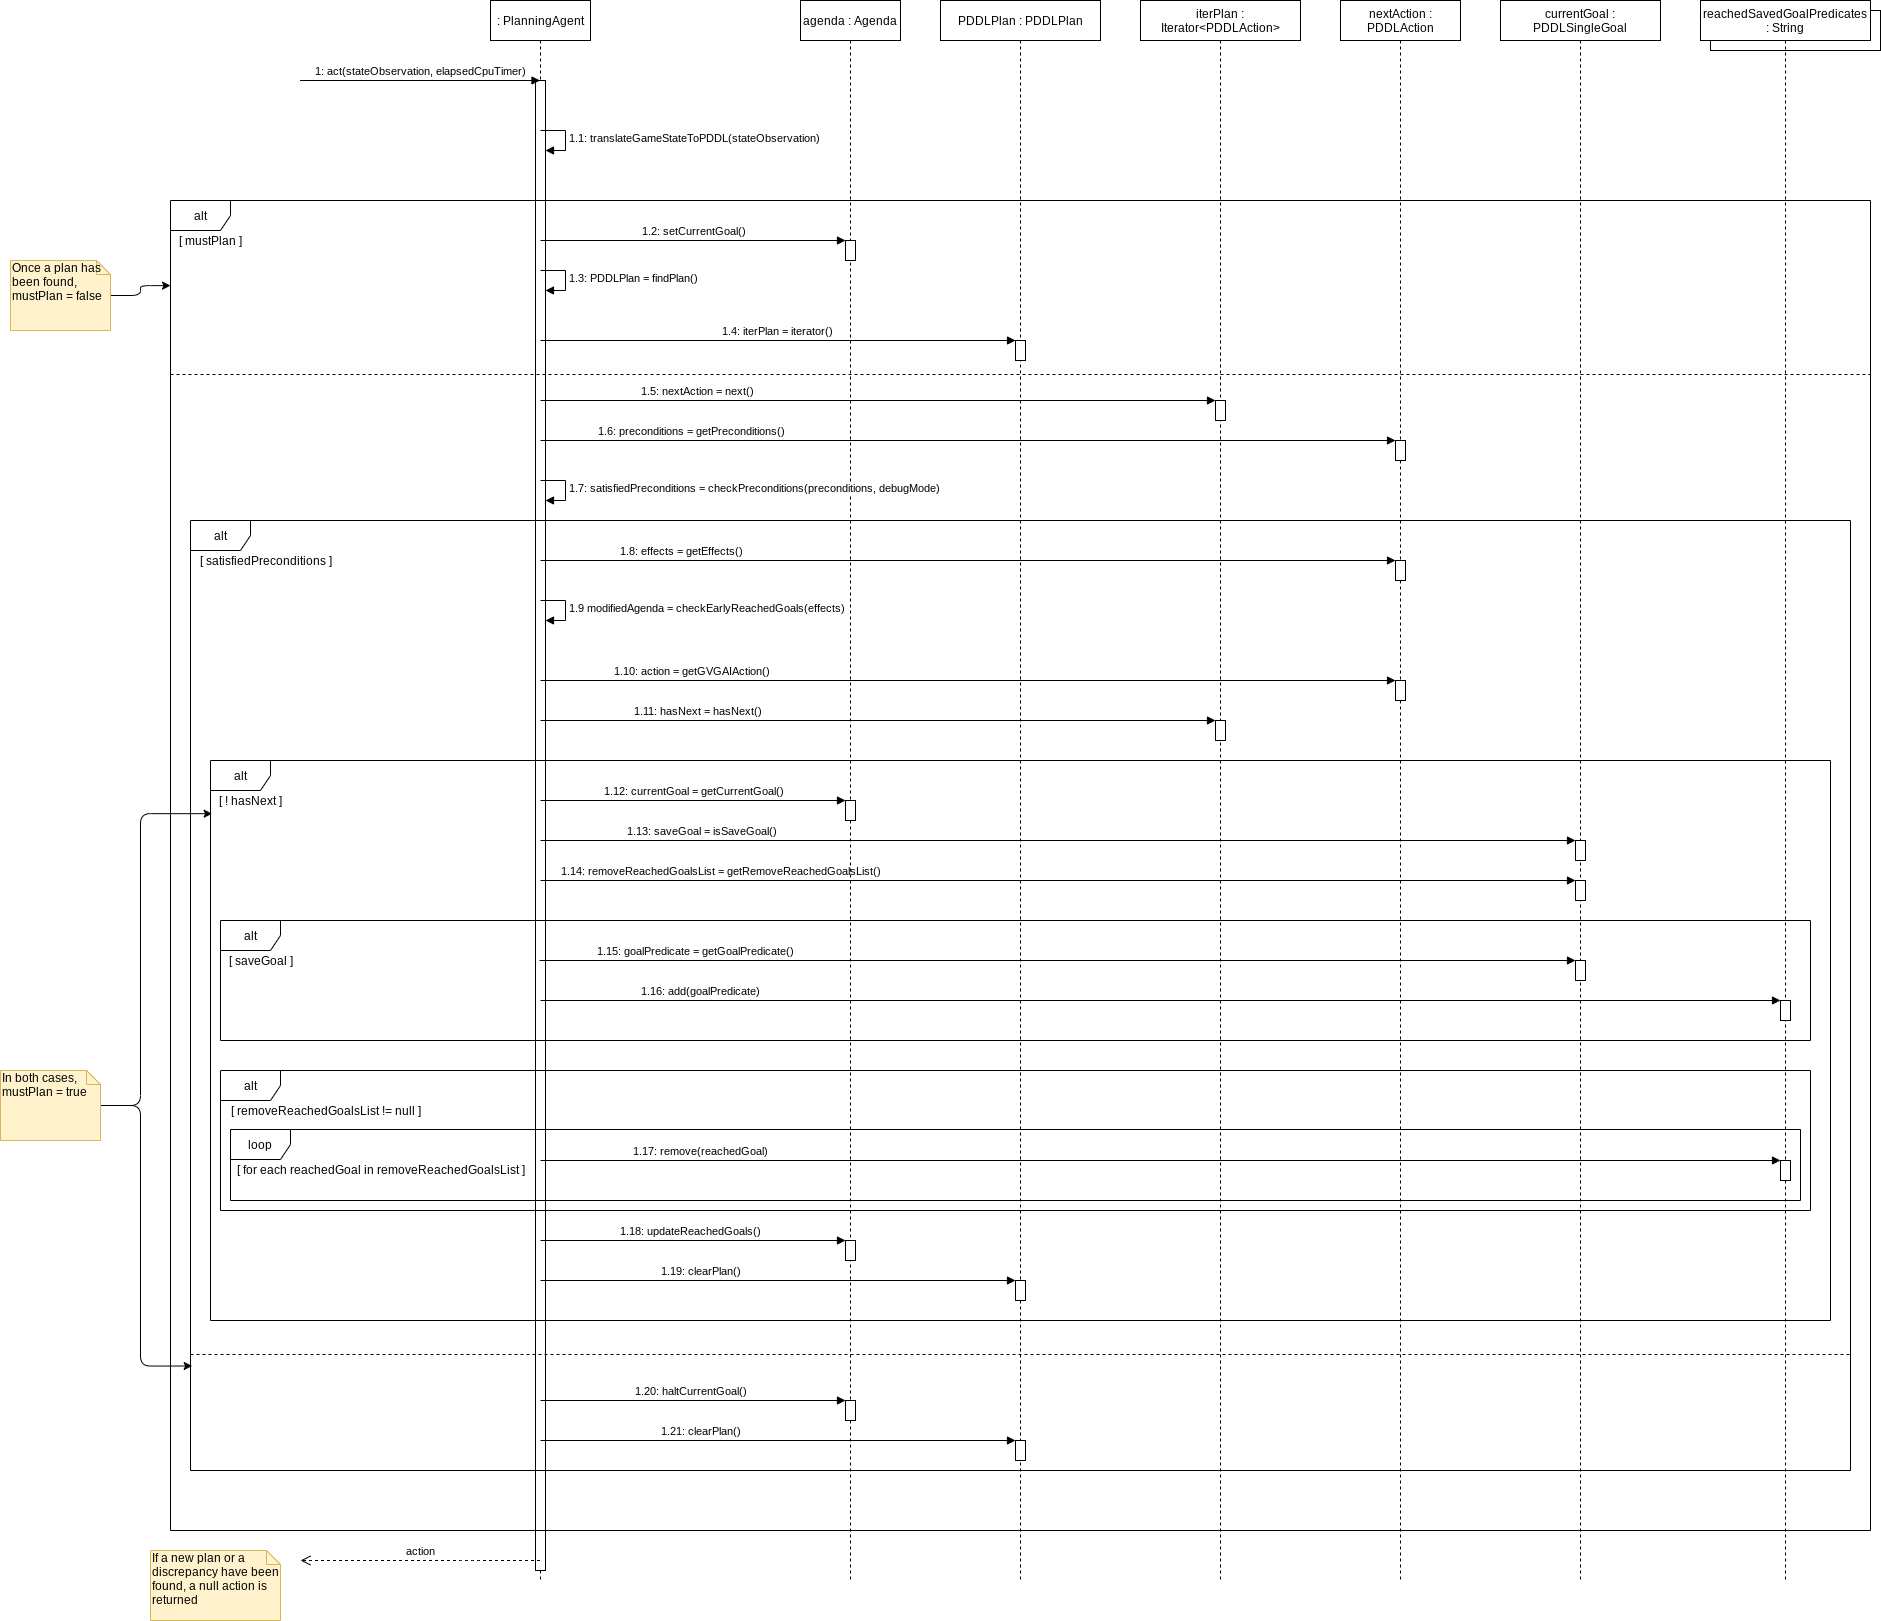
\includegraphics[scale=0.22]{img/CH07/sequence_diagram.png}
    \caption{Diagrama de secuencia del método \texttt{act()}.}
    \label{fig:sequence_diagram}
\end{figure}

\subsection{La clase \texttt{GameInformation}}

Esta clase representa la información del juego que se ha definido en el archivo de configuración.
Tiene exactamente los mismos campos que dicho archivo. Como son todos públicos, se puede instanciar
la clase y darle valores a dichos atributos. Sin embargo, es mucho más sencillo utilizar la funcionalidad
ofrecida por el paquete \texttt{org.yaml.snakeyaml} para crear directamente una nueva instancia con
la información del archivo.

\subsection{La clase \texttt{PDDLSingleGoal}}

La clase representa un objetivo a alcanzar. Los atributos que la componen son el predicado
objetivo (\texttt{goalPredicate}), la prioridad del objetivo (\texttt{priority}), un booleano
que indica si guardar o no el objetivo (\texttt{saveGoal}) y una lista de predicados a eliminar
cuando éste sea alcanzado (\texttt{removeReachedGoalsList}).

Para crear una instancia se podría llamar al constructor y usar los \textit{setters} para dar valores.
Sin embargo, en el sistema lo que se hace es cargar los objetivos directamente cuando se crea la
instancia de \texttt{GameInformation} a partir del archivo de configuración, ya que éstos aparecen reflejados
ahí.

\subsection{La clase \texttt{Agenda}}

Esta clase se encarga de gestionar los objetivos, de forma que es la que realiza la tarea del
\textbf{gestor de objetivos}. Para crear una instancia se necesita una lista de objetivos. Tal
y como pasaba antes, esto es muy fácil de hacer cuando se carga el archivo de configuración y
se obtiene dicha lista accediendo al atributo \texttt{goals} de la clase \texttt{GameInformation}.

Tal y como veíamos en el capítulo \ref{chap:desc}, un objetivo podía estar en diversos estados.
Para representar estos estados se tienen tres listas: una lista de objetivos no planificados
(\texttt{pendingGoals}), una lista de objetivos detenidos (\texttt{preemptedGoals}) y una lista
de objetivos alcanzados (\texttt{reachedGoals}). Adicionalmente, se tiene un atributo que representa
el estado de objetivo actual (\texttt{currentGoal}). Las listas \texttt{pendingGoals} y
\texttt{preemptedGoals} están ordenadas por prioridad.

Para seleccionar el objetivo actual se utiliza el método \texttt{setCurrentGoal}. El objetivo actual
se selecciona de la siguiente forma:

\begin{enumerate}[label=\arabic*º]
    \item Si \texttt{pendingGoals} contiene objetivos y \texttt{preemptedGoals} no, se selecciona
    el primero de \texttt{pendingGoals}.
    \item Si \texttt{preemptedGoals} contiene objetivos y \texttt{pendingGoals} no, se selecciona
    el primero de \texttt{preemptedGoals}.
    \item Si ambas listas contienen elementos, se comparan las prioridades del primer objetivo
    de cada lista y se escoge el de menor prioridad. En caso de empate, se decide escoger el
    objetivo de \texttt{pendingGoals} para así explorar nuevos objetivos.
    \item Si no quedan objetivos en ambas listas, significa que se han alcanzado todos los objetivos.
\end{enumerate}

El método \texttt{haltCurrentGoal} mueve el objetivo actual a la lista \texttt{preemptedGoals}
y establece que no hay ningún objetivo actual, de forma que se debe seleccionar uno nuevo.

\subsection{La clase \texttt{PDDLAction}}

Esta clase representa una instancia de una acción \texttt{PDDL}. Está formada por la acción instanciada
(\texttt{actionInstance}), la correspondiente acción \texttt{GVG-AI} (\texttt{GVGAIAction}), una lista
de precondiciones instanciadas (\texttt{preconditions}) una lista de efectos instanciados (\texttt{effects}).
Cuando se habla de instancias se hace referencia a que las variables han sido sustituidas por elementos
concretos del estado de observación actual del juego, en formato \texttt{PDDL} como es de suponer.
Las precondiciones y los efectos son proporcionados por el planificador como salida.

Una acción se crea cuando mientras se traduce el plan obtenido por el planificador. Dicho proceso
se realiza en el constructor de la clase. Por tanto, el constructor realiza parte del trabajo que realiza
el \textbf{traductor de planes}.

\subsection{La clase \texttt{PDDLEffect}}

Esta es una clase interna a \texttt{PDDLAction} y representa los efectos instanciados de una acción.
Un efecto consta de un predicado de efecto (\texttt{effectPredicate}) y de una lista de condiciones
(\texttt{conditions}). La existencia de condiciones implica que se trata de un efecto condicional,
siendo necesario por tanto que se cumplan las condiciones para que el efecto se lleve a cabo.

La existencia de una instancia de esta clase depende de una instancia de \texttt{PDDLAction}, ya
que si no existe una acción, no pueden existir efectos.

\subsection{La clase \texttt{PDDLPlan}}

Esta clase representa un plan traducido, o lo que es lo mismo, una secuencia de instancias de la
clase \texttt{PDDLAction}. Es el constructor de esta clase el que construye dicho plan, construyendo
cada acción de forma individual a partir de la respuesta del planificador. Además, el resultado obtenido
es posteriormente filtrado, de manera que las acciones nulas (aquellas que no tienen una correspondencia)
son eliminadas del plan. Por tanto, el constructor de la clase realiza parte del trabajo que realiza el
\textbf{traductor del plan}. El método \texttt{iterator} devuelve un iterador que permite recorrer el plan
de manera sencilla.

\section{Validación del \textit{software}}

Comprobar el correcto funcionamiento de \textit{software} de este tipo puede llegar a ser
complicado y tedioso, ya que implicaría tener que ejecutar cada vez una partida y comprobar qué
posibles errores se han producido a la hora de ejecutarlo o, en caso de que no se produzca ninguno,
comprobar que el resultado obtenido es el esperado.

Para simplificar todo el proceso, se han creado una serie de tests unitarios que comprueban
el correcto funcionamiento de las clases desarrolladas. De esta forma, antes incluso de
ejecutar un juego se puede llegar a asegurar el correcto funcionamiento del código implementado
y se pueden llegar a detectar errores que podrían afectar a su funcionamiento.

Dichos tests se ejecutan cuando se construye el archivo ejecutable del sistema, aunque también se
ha automatizado su ejecución por medio de plataformas de integración continua
(CI o \textit{Continuous Integration}) como por ejemplo serían \texttt{Travis CI} o las
recientemente creadas \texttt{GitHub Actions}, las cuales también permiten ejecutar tests.
De esta forma, cada vez que se haga un cambio en el repositorio se van a ejecutar los tests definidos,
con la ventaja además de que se pueden probar en múltiples sistemas operativos y versiones de éstos.
En este caso, se han realizado pruebas en \texttt{Ubuntu 16.04}, \texttt{Ubuntu 18.04}
y \texttt{Windows 10}. Desafortunadamente, no se han podido hacer pruebas en \texttt{macOS}
debido a problemas de estas plataformas a la hora de crear el entorno de pruebas.

Los tests creados realizan pruebas sobre toda la interfaz pública de las clases \texttt{Agenda},
\texttt{PDDLAction} (y por tanto también se testea la clase \texttt{PDDLEffect}), \texttt{PDDLPlan} y
\texttt{PDDLSingleGoal}. De esta forma se puede asegurar que las estructuras de datos se crean
de forma correcta y que los métodos implementados tienen el comportamiento esperado.

Para la clase \texttt{PlanningAgent} también se han creado una serie de tests que realizan
pruebas sobre una serie de métodos de la interfaz pública. Sin embargo, testear el método
\texttt{act} es complicado, ya que implicaría tener que crear una instancia de un juego
determinado, lo cual puede llegar a ser costoso. Para solventar eso, se han hecho pruebas
sobre los métodos públicos de la clase que intervienen en la ejecución de \texttt{act}. De esta
forma, si dichos métodos funcionan correctamente, se puede llegar a afirmar con bastante certeza
que el método tendrá el comportamiento esperado. Por tanto, para comprobar que esto es así bastaría
con realizar una ejecución con algún juego y comprobar el resultado. Como el resto de funcionalidades
han sido testeadas, se puede asegurar que su comportamiento va a ser el esperado y que no van a generar
errores durante la ejecución.
